\documentclass[conference]{IEEEtran}
\IEEEoverridecommandlockouts
\usepackage{tikz}
\usetikzlibrary{shapes.geometric, arrows, shapes.gates.logic.US, calc}
\usepackage{cite}
\usepackage{amsmath,amssymb,amsfonts}
\usepackage{algorithm}
\usepackage{algpseudocode}
\usepackage{graphicx}
\usepackage[OT1]{fontenc}
\usepackage{xcolor}
\usepackage{pgfplots}
\pgfplotsset{compat=1.9}

\def\BibTeX{{\rm B\kern-.05em{\sc i\kern-.025em b}\kern-.08em
    T\kern-.1667em\lower.7ex\hbox{E}\kern-.125emX}}

\newcommand\T{\rule{0pt}{2.6ex}}       % Top strut
\newcommand\B{\rule[-1.2ex]{0pt}{0pt}} % Bottom strut

\makeatletter

\begin{document}

%%%%%%%%%%%%%%%%%%%%%%%%%%%%%%%%%%%%%%%%%%%%%%%%%%%%%%%%%%%%%%%%%%%%%%%%%%%%%%%%%%%
%%%%%%%%%%%%%%%%%%%%%%%%%%%%%%%%%%%%%% TITLE %%%%%%%%%%%%%%%%%%%%%%%%%%%%%%%%%%%%%%
%%%%%%%%%%%%%%%%%%%%%%%%%%%%%%%%%%%%%%%%%%%%%%%%%%%%%%%%%%%%%%%%%%%%%%%%%%%%%%%%%%%

\title{Improving Placement in VLSI Design Process via Hybridization of Simulated Annealing and Genetic Algorithms \\}

%%%%%%%%%%%%%%%%%%%%%%%%%%%%%%%%%%%%%%%%%%%%%%%%%%%%%%%%%%%%%%%%%%%%%%%%%%%%%%%%%%%
%%%%%%%%%%%%%%%%%%%%%%%%%%%%%%%%%%%%% AUTHORS %%%%%%%%%%%%%%%%%%%%%%%%%%%%%%%%%%%%%
%%%%%%%%%%%%%%%%%%%%%%%%%%%%%%%%%%%%%%%%%%%%%%%%%%%%%%%%%%%%%%%%%%%%%%%%%%%%%%%%%%%

\author{\IEEEauthorblockN{Nada Adel\IEEEauthorrefmark{1}, Nader AbdAlGhani\IEEEauthorrefmark{2}, Nourhan Gamal\IEEEauthorrefmark{3} and Sarah Raafat\IEEEauthorrefmark{4}}
\IEEEauthorblockA{Computer Engineering Dept.,
Faculty of Engineering, Cairo University\\
Cairo, Egypt\\
\IEEEauthorrefmark{1}nadoza.98@gmail.com,
\IEEEauthorrefmark{2}nader\_abdelghani@hotmail.com,
\IEEEauthorrefmark{3}nourgamal1498@gmail.com,
\IEEEauthorrefmark{4}sararaafat1@yahoo.com}}


\maketitle

%%%%%%%%%%%%%%%%%%%%%%%%%%%%%%%%%%%%%%%%%%%%%%%%%%%%%%%%%%%%%%%%%%%%%%%%%%%%%%%%%%%
%%%%%%%%%%%%%%%%%%%%%%%%%%%%%%%%%%%% ABSTRACT %%%%%%%%%%%%%%%%%%%%%%%%%%%%%%%%%%%%%
%%%%%%%%%%%%%%%%%%%%%%%%%%%%%%%%%%%%%%%%%%%%%%%%%%%%%%%%%%%%%%%%%%%%%%%%%%%%%%%%%%%

\begin{abstract}

The simulated annealing algorithm is extensively used for cell placement in VLSI but its main downside is that it requires intensive computing to have optimum solutions in practical time. Genetic algorithms may get trapped in local minima, however, they traverse the solution space more rapidly. In this paper, simulated annealing and genetic algorithms are combined in order to achieve better solutions for VLSI cell placement. The genetic algorithm used is enhanced by taking the simulated annealing algorithm results as the initial population instead of generating random populations. Simulation outcome shows encouraging results in terms of overall wirelength.

\end{abstract}

%%%%%%%%%%%%%%%%%%%%%%%%%%%%%%%%%%%%%%%%%%%%%%%%%%%%%%%%%%%%%%%%%%%%%%%%%%%%%%%%%%%
%%%%%%%%%%%%%%%%%%%%%%%%%%%%%%%%%%%% KEY WORDS %%%%%%%%%%%%%%%%%%%%%%%%%%%%%%%%%%%%
%%%%%%%%%%%%%%%%%%%%%%%%%%%%%%%%%%%%%%%%%%%%%%%%%%%%%%%%%%%%%%%%%%%%%%%%%%%%%%%%%%%

\begin{IEEEkeywords}

Very-large-scale integration (VLSI), Standard cell placement, Computer-aided design (CAD), Simulated annealing (SA), Genetic algorithms (GA), Integrated circuits (ICs).

\end{IEEEkeywords}

%%%%%%%%%%%%%%%%%%%%%%%%%%%%%%%%%%%%%%%%%%%%%%%%%%%%%%%%%%%%%%%%%%%%%%%%%%%%%%%%%%%
%%%%%%%%%%%%%%%%%%%%%%%%%%%%%%%%%% INTRODUCTION %%%%%%%%%%%%%%%%%%%%%%%%%%%%%%%%%%%
%%%%%%%%%%%%%%%%%%%%%%%%%%%%%%%%%%%%%%%%%%%%%%%%%%%%%%%%%%%%%%%%%%%%%%%%%%%%%%%%%%%

\section{Introduction}

The result of the astronomical impact of the very large scale integration (VLSI) industry on the global economy and the extreme widespread use of electronic devices and equipment in various fields across the globe have led to the exponential increase in demand and sophistication of electronic devices. This, of course, goes along with Moore's law which refers to Gordon Moore's projection in 1965 that the number of transistors crammed in integrated circuits (ICs) doubles every two years, though their cost is halved. This increase in the number of transistors put in an IC comes at a cost which are the problems that arise during both the design process and the fabrication process of such intricate devices. This paper addresses the role of placement in the physical design process. Placement tools are used mainly for two things, the first is to place cells in a suitable way for the consequent routing process, and the second is to guide both synthesis and floorplanning processes. Over the years, placement has no longer become a fine-tunning tool used in physical design, but for that matter, it has become a notable contributor to the timing closure process results as well as being an overall major step in physical design. Conventionally, placement is divided into two subprocesses, global placement and detailed placement, however, the scope of this paper will focus exclusively on the former. Global placement aims to evenly and legally distribute the cells over the available placement region putting in mind cells relative positions to each other globally regardless of local problems that may arise, hence the name. This goal is achieved in favour of certain cost metrics such as overall wirelength and the time taken to achieve such a goal. The placement problem is to place the cells in such a way to achieve the best possible cost metrics. Much like the well-known travelling salesman problem and most, if not all, physical design problems, it is an NP-complete problem in combinatorial optimization. Most of the attempts at solving this problem use heuristic algorithms instead of the ineffective brute force trivial approach. Among those metaheuristics are simulated annealing which is popularly used in the optimization of this particular problem, and genetic algorithm which is used for optimization problems in general. In this paper, we implemented the best of both worlds to achieve overall better optimization in terms of wirelength and time.

%%%%%%%%%%%%%%%%%%%%%%%%%%%%%%%%%%%%%%%%%%%%%%%%%%%%%%%%%%%%%%%%%%%%%%%%%%%%%%%%%%%
%%%%%%%%%%%%%%%%%%%%%%%%%%%%%%%%%% RELATED WORK %%%%%%%%%%%%%%%%%%%%%%%%%%%%%%%%%%%
%%%%%%%%%%%%%%%%%%%%%%%%%%%%%%%%%%%%%%%%%%%%%%%%%%%%%%%%%%%%%%%%%%%%%%%%%%%%%%%%%%%

\section{Related Work}

As already stated, the placement problem is an NP-complete problem where its optimum solution can be found by trying all possible cells configurations, but due to the tremendous number of cells that exist in almost all VLSI designs which range from millions to billions of cells, it would be utterly impractical to compute every possible configuration in order to find the fittest one. Because of this nature, previous literature made significant improvements in terms of solution fitness and the amount of time consumed through using heuristic techniques such as simulated annealing used in \cite{b7}, \cite{b10}, \cite{b11}, \cite{b12}, \cite{b13} and \cite{b14}, min-cut placement algorithm used in \cite{b1} and \cite{b15} and genetic algorithms used in \cite{b2}, \cite{b3} and \cite{b7}. However, optimizing placement algorithms isn't limited to heuristic approaches only as others have used different approaches to achieve solid results. For instance, Natarajan et al \cite{b8} used an analytical placement algorithm that is based on the quadratic placement approach.

\subsection{Simulated Annealing}

Simulated annealing is one of the popular and most effective algorithms among all placement algorithms, in fact, it is generally used as an optimization technique for combinatorial problems. The basic idea of this method comes from the annealing treatment in metallurgy. Annealing in metallurgy is used to accomplish a crystalline lattice structure of the particles of solid metal as it reflects a minimum energy state for the solid. This is achieved by heating the metal in a heat bath until it reaches a temperature named the initial temperature of the annealing process at which all particles are randomly arranged, then whenever the metal reaches thermal equilibrium the temperature is reduced gradually according to a cooling schedule otherwise the resulting crystal will not mirror a minimum energy state. This analogy applies to the simulated annealing metaheuristic where an initial value of temperature $T$ is set and at each iteration, the positions of the cells get scrambled around legal regions then the cost function $C$ is measured, a result is accepted whenever it leads to a decreasing cost function, however, if a result leads to an increasing cost function, it is accepted if and only if the move has a probability greater than a random value between $0$ and $1$. The probability function is defined as follows:

    \begin{equation}
        P = e^{-\Delta C/T}
    \end{equation}

At the end of each iteration, the temperature value decreases by multiplying it by a cooling factor which is less than $1$. This process iterates until the temperature goes below $1$. It is clear that the performance of this algorithm is based upon four parameters\slash steps:

\subsubsection{Initial Configuration}
In this step, the individual cells are extracted from the circuit and for each cell, the inputs and outputs are determined. The following diagram and table show the circuit is decomposed.
\begin{figure}[H]
    \centering
    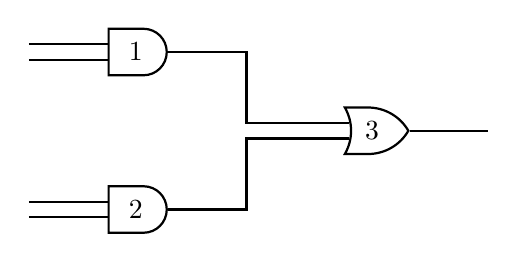
\begin{tikzpicture}[thick, scale = 2]
        \node[and gate US, draw, rotate=0, logic gate inputs=nn] at (0,1) (and1) {1};
        \node[and gate US, draw, rotate=0, logic gate inputs=nn] at (0,0) (and2) {2};
        \node[or gate US, draw, rotate=0, logic gate inputs=nn] at ($(and2) + (1.5, 0.5)$) (or1) {3};

        \draw ($(and1.input 1) + (-0.5, 0)$) -- (and1.input 1);
        \draw ($(and1.input 2) + (-0.5, 0)$) -- (and1.input 2);
        \draw ($(and2.input 1) + (-0.5, 0)$) -- (and2.input 1);
        \draw ($(and2.input 2) + (-0.5, 0)$) -- (and2.input 2);
    
        \draw (and1.output) -- ([xshift=0.5cm]and1.output) |- (or1.input 1);
        \draw (and2.output) -- ([xshift=0.5cm]and2.output) |- (or1.input 2);
    
        \draw (or1.output) -- ++ (0.5,0);
    \end{tikzpicture}
    \caption{Sample circuit diagram}
\end{figure}

\begin{table}[H]
    \caption{Sample Cells Data}
    \centering
     \begin{tabular}{||c c c||} 
     \hline
     \textit{\textbf{Cell}} & \textit{\textbf{Input}} & \textit{\textbf{Output}} \T \B \\ 
     \hline
     \hline
     1 & - & 3 \T \B \\ 
     \hline
     2 & - & 3 \T \B \\
     \hline
     3 & 1 & - \T \B \\
     \hline
     3 & 2 & - \T \B \\
     \hline
     \end{tabular}
     \label{table1}
\end{table}

At this step, the total wirelength of cells interconnections will most likely be large due to them being placed randomly. Hence the presence of the rest of the subsequent procedures which aim to achieve the optimal placement of the cells.
\medskip

\subsubsection{Move Generation Function}

At each iteration, cells are rearranged to generate a new placement configuration of the cells. To do so, there are two possible strategies used:
\begin{itemize}
    \item Move cells randomly to new legal positions 
    \item Swap the positions of each two cells
\end{itemize}
\medskip

\subsubsection{Cost Function}

The cost function consists of two terms as follows:
\begin{equation}
    C = C_{1} + C_{2}
\end{equation}
Where $C_{1}$ is the measure of the total wirelength and $C_{2}$ is the measure of total overlap of the chip which is sometimes neglected as in our case but it is used in other papers \cite{b16} nevertheless.

Let $d_{h}^{ij}$ $d_{v}^{ij}$ be the horizontal and the vertical distance between cell $i$ and its $j^{th}$ out cell respectively, the total wire length of the chip can be expressed as the following equation 
\begin{equation}
    C_{1} = \sum_{i=cell}^{n} \sum_{j=out cell}^{n} (d_{h}^{ij} + d_{v}^{ij})
\end{equation}
Where $n$ is the total number of cells in the chip. In case of the second term $C_{2}$, whenever two cells are swapped, they might overlap, therefore, $O_{ij}$ indicates the overlap between cell $i$ and cell $j$, this overlap is undesirable and it negatively affects the cost function by increasing its value by the term $C_{2}$ which is the summation of each overlap value squared.
\begin{equation}
    C_{2} = \sum_{i!=j} (O_{ij}^{2})
\end{equation}
The cost function is calculated at each iteration after generating a new cells layout.
\medskip

\subsubsection{Annealing Schedule}

At first, the temperature $T$ is initialized to a very large value, and at every iteration, the temperature is reduced using the following equation:
\begin{equation}
    T = \alpha*T
\end{equation}
Where $\alpha$ is the cooling rate. In our case, it has a constant value of $0.995$. Yet, it can be set dynamically in the following fashion: Initially, it is set to a small value which contributes to the rapid decrease in temperature, then in the middle of the annealing process the temperature is reduced slowly via a larger cooling rate value. When the temperature is relatively low, the temperature decreases rapidly again until the stopping condition which is when the temperature falls below $1$ is met.

\medskip

\begin{algorithm}[H]
    \caption{Simulated Annealing}
    \begin{algorithmic}[1]
    \renewcommand{\algorithmicrequire}{\textbf{Input:}}
    \renewcommand{\algorithmicensure}{\textbf{Output:}}
    \Ensure  Optimized solution $S$
       \State Create an initial solution $x$
     \State Set $\alpha \in (0,1)$, temperature $T$
     \State Set $S = x$
     \While{Stopping criterion is NOT satisfied}
       \State $x^{'} = $ a neighbouring solution
       \State Calculate $C(x^{'})$
       \State Calculate $\Delta C = C(x^{'}) - C(x)$
       \If{$\Delta C < 0$}
           \State $x = x^{'}$
           \If{$C(x) < C(S)$}
               \State $S = x$
           \EndIf
       \ElsIf{$rand(0,1) < e^{-\Delta C/T}$}
           \State $x = x^{'}$
       \EndIf
       \State $T = T * \alpha$
     \EndWhile
    \State \textbf{return} $S$
    \end{algorithmic} 
\end{algorithm}

There is no doubt that this widely-used algorithm yields excellent results, as a matter of fact, it can produce the global optimum result given enough time which makes it a solid contender for solving the end-case placement problem. Though it still has its set of drawbacks. For instance, it is extremely slow especially if rooting for the global optimum solution, not to mention that it suffers hugely if there is a scarce number of local minima.

\subsection{Genetic Algorithm}

Genetic algorithms are metaheuristics based on the concepts of Charles Darwin's theory of biological evolution. Its idea is powered by the natural principle known as “survival of the fittest” where the fittest individuals have the highest probability of survival and to pass their genes to their offspring for further reproduction. On the other hand, the less fit individuals have the highest probability to die out. This resemblance is commonly used for creating optimization algorithms for combinatorial problems. But given the characteristics of the VLSI design placement problem, a genetic algorithm can also be employed to solve it as in \cite{b2}. Genetic algorithms effectiveness is defined by the following parameters:

\subsubsection{Initial Population}

The initial population individuals are a subset of the solution space. They represent the first generation and they are usually created randomly. However, by intuition, the better the first generation is the lesser time consumed by the algorithm to find better individuals. Each individual is represented by a chromosome which reflects its information in an appropriate encoding.

\medskip

\subsubsection{Crossover}

Crossover is quite similar to sexual reproduction in biology as it is used for combining the genetic information of two individuals "parents" of the current population to generate a new solution. Solutions are usually mutated before being added to the new population.

\medskip

\subsubsection{Mutation}

The mutation process operates on the output of the crossover process. It introduces new variations in their chromosomes in an attempt to span the whole solution space.

\medskip

\subsubsection{Selection}

Selection is the criteria with which the selection of the fittest individuals of the generated offspring for later reproduction occurs. It is usually implemented as a fitness function that is evaluated for each individual.

\medskip

\begin{algorithm}[H]
\caption{Genetic Algorithm Pseudo Code}
    \begin{algorithmic}[1]
    \renewcommand{\algorithmicrequire}{\textbf{Input:}}
    \renewcommand{\algorithmicensure}{\textbf{Output:}}
    \Ensure  The fittest Individual according to a certain criteria
        \State Randomly generate an initial population
        \State Evaluate the fitness of each individual of the population
        \While{The fittest Individual NOT found}
            \State Select the fittest individuals
            \State Generate new individuals using the crossover operator
            \State Mutate the new individuals
            \State Evaluate the fitness of the new individuals
            \State Replace the worst individuals of the population with the best new individuals
        \EndWhile
        \State \textbf{return} The fittest individual
    \end{algorithmic}
\end{algorithm}

From \cite{b7}, we can deduce that as much as genetic algorithms offer lots of advantages like having relatively easy implementations, being faster than simulated annealing to finding fit solutions and being able to span the solution space more rapidly. But despite those benefits, they have some hindering limitations. For example, they cannot find the exact minima value despite spanning most of the solution space quickly and they may also be trapped at local minima.

%%%%%%%%%%%%%%%%%%%%%%%%%%%%%%%%%%%%%%%%%%%%%%%%%%%%%%%%%%%%%%%%%%%%%%%%%%%%%%%%%%%
%%%%%%%%%%%%%%%%%%%%%%%%%%%%%%%% PROPOSED APPROACH %%%%%%%%%%%%%%%%%%%%%%%%%%%%%%%%
%%%%%%%%%%%%%%%%%%%%%%%%%%%%%%%%%%%%%%%%%%%%%%%%%%%%%%%%%%%%%%%%%%%%%%%%%%%%%%%%%%%

\section{Proposed Approach}

As already introduced, both the simulated annealing and genetic algorithms have their set of benefits and shortcomings. This paper approach tries to compensate each algorithm drawback with the advantage of the other. The role of the simulated annealing algorithm in our approach is to generate the initial population of the genetic algorithm used, as having an already-improved initial population will prevent the genetic algorithm from getting trapped in local minima. On the other side of the coin, the genetic algorithm spans the solution space in parallel via its population, which is much faster than the sequential spanning done by the simulated annealing algorithm. The proposed algorithm runs the simulated annealing algorithm on random placement configurations with a temperature value directly proportional to the number of cells in the input circuit to generate output configurations equal to the number of individuals in the initial population of the genetic algorithm. At the receiving end, the genetic algorithm evaluates each individual of the initial population according to the fitness function which sorts them with respect to their total wirelength, the shorter, the better. The crossover process is done by creating a new child placement configuration where each cell in this new placement is taken either from the first or the second parent while making sure that the cell taken at each crossover iteration does not coincide with another cell at the same coordinates. After the crossover process is executed between all the available cells, the generated configuration is mutated by swapping two randomly-chosen cells.

\begin{algorithm}[H]
    \caption{Proposed Algorithm}
    \begin{algorithmic}[1]
    \renewcommand{\algorithmicrequire}{\textbf{Input:}}
    \renewcommand{\algorithmicensure}{\textbf{Output:}}
    \Require Circuit $C_{o}$
    \Ensure  Optimized placement configuration $\eta$
    \State Generate an initial random cells placement $P$
    \While{Population $\sigma$ is NOT filled completely}
        \State Set $\alpha = 0.995$
        \State Set temperature $T = 2 * number\; of\; cells\; of\; C_{o}$
        \State Set optimized circuit configuration $\Phi = P$
        \While{$T > 1$}
        \State $P^{'} = $ randomly generated cells placement
        \State $\Delta C = wirelength(P^{'}) - wirelength(P)$
        \If{$\Delta C < 0$}
            \State $P = P^{'}$
            \If{$wirelength(P) < wirelength(\Phi)$}
                \State $\Phi = P$
            \EndIf
        \ElsIf{$rand(0,1) < e^{-\Delta C/T}$}
            \State $P = P^{'}$
        \EndIf
        \State $T = T * \alpha$
        \EndWhile
        \State \textbf{Append} $\Phi$ to $\sigma$
    \EndWhile
    \While{The termination condition is NOT satisfied}
        \State Sort $\sigma$ in descending order by the fitness level
        \State $\sigma^{*} = crossover(\sigma)$
        \State $\sigma^{*} = mutation(\sigma^{*})$
        \algrenewcommand\algorithmicfor{\textbf{foreach}}
        \For{$\sigma^{*}_{i} \in \sigma^{*}$}
            \State Evaluate $\sigma^{*}_{i}$ fitness level
        \EndFor
        \State $\sigma = \sigma^{*}$
    \EndWhile
    \State $\eta = $ the fittest individual of $\sigma$
    \State \textbf{return} $\eta$
    \end{algorithmic} 
\end{algorithm}

%%%%%%%%%%%%%%%%%%%%%%%%%%%%%%%%%%%%%%%%%%%%%%%%%%%%%%%%%%%%%%%%%%%%%%%%%%%%%%%%%%%
%%%%%%%%%%%%%%%%%%%%%%%%%%%%%% EXPERIMENTAL ANALYSIS %%%%%%%%%%%%%%%%%%%%%%%%%%%%%%
%%%%%%%%%%%%%%%%%%%%%%%%%%%%%%%%%%%%%%%%%%%%%%%%%%%%%%%%%%%%%%%%%%%%%%%%%%%%%%%%%%%

\section{Experimental Analysis}

%%%%%%%%%%%%%%%%%%%%%%%%%%%%%%%%%%%%%%%%%%%%%%%%%%%%%%%%%%%%%%%%%%%%%%%%%%%%%%%%%%%
%%%%%%%%%%%%%%%%%%%%%%%%%%%%%%%%%%% ASSUMPTIONS %%%%%%%%%%%%%%%%%%%%%%%%%%%%%%%%%%%
%%%%%%%%%%%%%%%%%%%%%%%%%%%%%%%%%%%%%%%%%%%%%%%%%%%%%%%%%%%%%%%%%%%%%%%%%%%%%%%%%%%

\subsection{Assumptions}

The proposed algorithm is software simulated using a program written in Java. This program simulates a $10*10$ grid on which cells are placed randomly. Cells are assumed to be identical. Each cell occupies a single unit of space on the grid and each cell has the same number of input and output ports which are $1$ and $2$ respectively. Cells input and output interconnections are mapped randomly, too, but under the condition that every cell is connected to only $2$ other cells.

%%%%%%%%%%%%%%%%%%%%%%%%%%%%%%%%%%%%%%%%%%%%%%%%%%%%%%%%%%%%%%%%%%%%%%%%%%%%%%%%%%%
%%%%%%%%%%%%%%%%%%%%%%%%%%%%%%%%%%%%%%% I/O %%%%%%%%%%%%%%%%%%%%%%%%%%%%%%%%%%%%%%%
%%%%%%%%%%%%%%%%%%%%%%%%%%%%%%%%%%%%%%%%%%%%%%%%%%%%%%%%%%%%%%%%%%%%%%%%%%%%%%%%%%%

\subsection{Experimental Scheme}

On one hand, the input arguments to the proposed algorithm implementation are the number of cells in the circuit with a maximum value of 52 and the population size used in the genetic algorithm. On the other hand, output parameters are the initial placement wirelength, the results of the simulated annealing algorithm runs, the result of a regular genetic algorithm with a randomly generated population, and finally, the result of the proposed algorithm.

%%%%%%%%%%%%%%%%%%%%%%%%%%%%%%%%%%%%%%%%%%%%%%%%%%%%%%%%%%%%%%%%%%%%%%%%%%%%%%%%%%%
%%%%%%%%%%%%%%%%%%%%%%%%%%%%%%% PERFORMANCE METRICS %%%%%%%%%%%%%%%%%%%%%%%%%%%%%%%
%%%%%%%%%%%%%%%%%%%%%%%%%%%%%%%%%%%%%%%%%%%%%%%%%%%%%%%%%%%%%%%%%%%%%%%%%%%%%%%%%%%

\subsection{Performance Metrics}

The total wirelength and the time consumed finding the optimum solution are usually the chosen metrics whenever it comes to performance evaluation of placement algorithms. Due to the dependability of the time consumed by the machines on which algorithms are run, only the total wirelength is chosen.

%%%%%%%%%%%%%%%%%%%%%%%%%%%%%%%%%%%%%%%%%%%%%%%%%%%%%%%%%%%%%%%%%%%%%%%%%%%%%%%%%%%
%%%%%%%%%%%%%%%%%%%%%%%%%%%%%%%%%%% COMPARISONS %%%%%%%%%%%%%%%%%%%%%%%%%%%%%%%%%%%
%%%%%%%%%%%%%%%%%%%%%%%%%%%%%%%%%%%%%%%%%%%%%%%%%%%%%%%%%%%%%%%%%%%%%%%%%%%%%%%%%%%

\subsection{Performance Comparisons}

Insert experiments comparisons here

%%%%%%%%%%%%%%%%%%%%%%%%%%%%%%%%%%%%%%%%%%%%%%%%%%%%%%%%%%%%%%%%%%%%%%%%%%%%%%%%%%%
%%%%%%%%%%%%%%%%%%%%%%%%%%%%%%%%%%% OBSERVATION %%%%%%%%%%%%%%%%%%%%%%%%%%%%%%%%%%%
%%%%%%%%%%%%%%%%%%%%%%%%%%%%%%%%%%%%%%%%%%%%%%%%%%%%%%%%%%%%%%%%%%%%%%%%%%%%%%%%%%%

\subsection{Observation}

Insert observation here


%%%%%%%%%%%%%%%%%%%%%%%%%%%%%%%%%%%%%%%%%%%%%%%%%%%%%%%%%%%%%%%%%%%%%%%%%%%%%%%%%%%
%%%%%%%%%%%%%%%%%%%%%%%%%%%%%%%%%%% CONCLUSION %%%%%%%%%%%%%%%%%%%%%%%%%%%%%%%%%%%%
%%%%%%%%%%%%%%%%%%%%%%%%%%%%%%%%%%%%%%%%%%%%%%%%%%%%%%%%%%%%%%%%%%%%%%%%%%%%%%%%%%%

\section{Conclusion and Future Work}

Insert conclusion and future work here

%%%%%%%%%%%%%%%%%%%%%%%%%%%%%%%%%%%%%%%%%%%%%%%%%%%%%%%%%%%%%%%%%%%%%%%%%%%%%%%%%%%
%%%%%%%%%%%%%%%%%%%%%%%%%%%%%%%%%%%% REFERENCES %%%%%%%%%%%%%%%%%%%%%%%%%%%%%%%%%%%
%%%%%%%%%%%%%%%%%%%%%%%%%%%%%%%%%%%%%%%%%%%%%%%%%%%%%%%%%%%%%%%%%%%%%%%%%%%%%%%%%%%

\begin{thebibliography}{00}

\bibitem{b1} Saab, Youssef, ``A fast clustering-based min-cut placement algorithm with simulated-annealing performance'', \textit{VLSI Design}, vol. 5, no. 1, 1996, pp. 37-48.

\bibitem{b2} H. Esbensen, ``A genetic algorithm for macro cell placement'', \textit{European Design Automation Conference}, Hamburg, Germany, 1992, pp. 52-57.

\bibitem{b3} K. Shahookar and P. Mazumder, ``GASP-a genetic algorithm for standard cell placement'', \textit{Proceedings of the European Design Automation Conference}, Glasgow, UK, 1990, pp. 660-664.

\bibitem{b4} J. Vygen, ``Algorithms for detailed placement of standard cells'', \textit{Proceedings Design, Automation and Test in Europe}, Paris, France, 1998, pp. 321-324.

\bibitem{b5} Min Pan, N. Viswanathan and C. Chu, ``An efficient and effective detailed placement algorithm'', \textit{ICCAD-2005. IEEE/ACM International Conference on Computer-Aided Design, 2005}, San Jose, CA, USA, 2005, pp. 48-55.

\bibitem{b6} Z. Jiang, H. Chen, T. Chen and Y. Chang, ``Challenges and Solutions in Modern VLSI Placement'', \textit{2007 International Symposium on VLSI Design, Automation and Test (VLSI-DAT)}, Hsinchu, 2007, pp. 1-5.

\bibitem{b7} Elhaddad, Younis, ``Combined simulated annealing and genetic algorithm to solve optimization problems'', \textit{World Academy of Science, Engineering and Technology}, 2012.

\bibitem{b8} N. Viswanathan and C. C. -. Chu, ``FastPlace: efficient analytical placement using cell shifting, iterative local refinement,and a hybrid net model'', \textit{IEEE Transactions on Computer-Aided Design of Integrated Circuits and Systems}, vol. 24, no. 5, May 2005, pp. 722-733.

\bibitem{b9} D. Zaporozhets, D. Zaruba and N. Kulieva, ``Hybrid heuristic algorithm for VLSI placement'', \textit{2019 International Russian Automation Conference (RusAutoCon)}, Sochi, Russia, 2019, pp. 1-5.

\bibitem{b10} R. F. Hentschke and R. A. D. L. Reis, ``Improving simulated annealing placement by applying random and greedy mixed perturbations [IC layout]'', \textit{16th Symposium on Integrated Circuits and Systems Design, 2003. SBCCI 2003. Proceedings}, Sao Paulo, Brazil, 2003, pp. 267-272.

\bibitem{b11} K. Vorwerk, A. Kennings and J. W. Greene, ``Improving Simulated Annealing-Based FPGA Placement With Directed Moves'', \textit{IEEE Transactions on Computer-Aided Design of Integrated Circuits and Systems}, vol. 28, no. 2, Feb. 2009, pp. 179-192.

\bibitem{b12} Atanu Roy, Karthik Ganesan Pillai, ``Parallel simulated annealing for VLSI
cell placement problem'', 2009.

\bibitem{b13} J. A. Chandy and P. Banerjee, ``Parallel simulated annealing strategies for VLSI cell placement'', \textit{Proceedings of 9th International Conference on VLSI Design}, Bangalore, India, 1996, pp. 37-42.

\bibitem{b14} J. W. Greene and K. J. Supowit, ``Simulated annealing without rejected moves'', \textit{IEEE Transactions on Computer-Aided Design of Integrated Circuits and Systems}, vol. 5, no. 1, January 1986, pp. 221-228.

\bibitem{b15} A. B. Kahng and S. Reda, ``Wirelength minimization for min-cut placements via placement feedback'', \textit{IEEE Transactions on Computer-Aided Design of Integrated Circuits and Systems}, vol. 25, no. 7, July 2006, pp. 1301-1312.

\bibitem{b16} Shahookar, K. and Mazumder, ``VLSI cell placement techniques'', \textit{ACM Computing Surveys}, vol. 23, no. 2, pp. 145-220.

\end{thebibliography}

\end{document}
